% **************************************************
% Document Class Definition
% **************************************************
\documentclass[%
    paper=A4,               % paper size --> A4 is default in Germany
    twoside=true,           % onesite or twoside printing
    openright,              % doublepage cleaning ends up right side
    parskip=full,           % spacing value / method for paragraphs
    chapterprefix=true,     % prefix for chapter marks
    11pt,                   % font size
    headings=normal,        % size of headings
    bibliography=totoc,     % include bib in toc
    listof=totoc,           % include listof entries in toc
    titlepage=on,           % own page for each title page
    captions=tableabove,    % display table captions above the float env
    chapterprefix=false,    % do not display a prefix for chapters
    appendixprefix=false,   % but display a prefix for appendix chapter
    draft=false,            % value for draft version
]{scrreprt}%


% **************************************************
% Setup YOUR thesis document in this file !
% **************************************************
\input{my-thesis-setup}


% **************************************************
% Document CONTENT
% **************************************************
\begin{document}

% --------------------------
% rename document parts
% --------------------------
%\renewcaptionname{ngerman}{\figurename}{Abb.}
%\renewcaptionname{ngerman}{\tablename}{Tab.}
\renewcaptionname{english}{\figurename}{Fig.}
\renewcaptionname{english}{\tablename}{Tab.}

% --------------------------
% Front matter
% --------------------------
\pagenumbering{roman}			% roman page numbing (invisible for empty page style)
\pagestyle{empty}				% no header or footers
\input{content/titlepages}		% INCLUDE: all titlepages
\cleardoublepage

\pagestyle{plain}				% display just page numbers
% !TEX root = ../main.tex
%
\pdfbookmark[0]{Abstract}{Abstract}
\chapter*{Abstract}
\label{sec:abstract}
\vspace*{-10mm}

Standard uncertainty estimation in Large Language Models (LLMs) 
relies on single, fixed probability distributions. This 
``point-estimate'' approach often conflates benign linguistic 
diversity with factual ignorance, failing to reliably quantify 
uncertainty.
In this thesis, we introduce \textit{Credal Semantic Entropy},
a rigorous framework grounded in Imprecise Probabilities. 
We propose a method to construct Credal Sets---convex sets of 
probability distributions---based on the statistical notion of 
relative likelihood. Instead of relying on a single temperature,
we identify a set of statistically valid temperatures that
maximize the likelihood of calibration data. We cluster generated
sequences by semantic meaning and derive interval-valued
probabilities, computing the Upper Semantic Entropy to capture
a worst-case estimate of uncertainty.
We empirically evaluate our approach on the CoQA benchmark using
the OPT-6.7B model. While theoretically robust, experiments 
reveal that the credal framework is highly sensitive to relative
likelihood thresholds ($\alpha$-cuts). Under our tested 
configurations, single-point baselines outperform Credal Semantic 
Entropy in uncertainty estimation (measured via AUROC).
%This thesis lays the foundational groundwork for
%applying credal uncertainty estimation to autoregressive language
%models, opening new avenues for future research.

\iffalse
Accurately quantifying uncertainty in Large Language Models (LLMs) is 
crucial for their deployment in safety-critical domains. However, 
standard uncertainty estimation methods typically rely on a single 
probability distribution defined by fixed decoding hyperparameters. 
We argue that this "point-estimate" approach fails to adequately 
capture epistemic uncertainty, often conflating benign linguistic 
diversity with factual ignorance.
In this thesis, we introduce \textit{Credal Semantic Entropy}, a 
rigorous framework for hallucination detection grounded in the theory 
of Imprecise Probabilities. We propose a method to construct Credal 
Sets—convex sets of probability distributions—based on the statistical 
notion of relative likelihood. Instead of relying on a single 
temperature, we identify a set of statistically valid temperatures 
that maximize the likelihood of calibration data. We then aggregate 
generated sequences into semantic clusters and derive interval-valued 
probabilities  for each meaning. By computing the Upper Semantic 
Entropy over these intervals, we obtain a worst-case estimate of 
uncertainty.
\fi

\vspace*{20mm}
		% INCLUDE: the abstracts (english and german)
\cleardoublepage
%
% Acknowledgement is optional
% !TEX root = ../main.tex
%
\pdfbookmark[0]{Acknowledgement}{Acknowledgement}
\chapter*{Acknowledgement}
\label{sec:acknowledgement}
\vspace*{-10mm}

Large Language Models (LLMs) were used to support several stages of this work. Their assistance included co-coding and troubleshooting during development, helping to brainstorm approaches and refine ideas, and providing guidance for resolving code bugs. LLMs were also used to improve the clarity of written content by correcting spelling, grammar, and phrasing. All substantive decisions, analysis, and final interpretations were made by the author.
 % INCLUDE: acknowledgement
% \cleardoublepage
%
\currentpdfbookmark{\contentsname}{toc}
\setcounter{tocdepth}{2}		% define depth of toc
\tableofcontents				% display table of contents
\cleardoublepage

% --------------------------
% Body matter
% --------------------------
\pagenumbering{arabic}			% arabic page numbering
\setcounter{page}{1}			% set page counter
\pagestyle{scrheadings} 	% fancy header and footer

\input{content/chapter-introduction}   % INCLUDE: introduction
\input{content/chapter-background}     % INCLUDE: background
\input{content/chapter-related-work}   % INCLUDE: related work
% !TEX root = ../main.tex
%
\chapter{Methodology: Credal Semantic Entropy via Temperature Scaling}
\label{sec:methodology}
This chapter introduces a novel methodology that constructs a 
credal set for LLMs by dynamically scaling the decoding temperature.
By treating the temperature hyperparameter as a continuous parameter 
space and applying the statistical principles of relative likelihood,
we systematically filter out implausible distributions. We then 
extend semantic entropy to operate over this credal set, yielding
robust upper and lower uncertainty bounds that serve as a signal 
for hallucination detection.

\section{Overview of the Pipeline}
\label{sec:methodology:overview}
Our proposed methodology, which we term Credal Semantic Entopy,
works for a given input prompt $x$ (a question and optional context),
in four sequential stages:

\begin{enumerate}
    \item \textbf{Valid Temperature Selection (The $\alpha$-cut)}:
	Before generation, we must determine which temperatures
	produce statistically valid probability distributions. 
	Using a labeled dataset, we evaluate the model's 
	average Negative Log-Likelihood (NLL) as shown in 
	\ref{eq:average_nll}
	across a discrete grid of temperatures. 
	We identify the optimal temperature
	that minimizes the average NLL and compute the relative 
	likelihood for all temperatures. The $\alpha$-cut is 
	constructed by all temperatures with a relative likelihood
	greater or equal than $\alpha$.

    \item \textbf{Generation and Semantic Clustering}:
	Using the prompt $x$, the LLM generates multiple candidate
	responses at every valid temperature in the $\alpha$-cut.
	We cluster these generated sequences by their meaning
	over all valid temperatures. 

    \item \textbf{Computation of Cluster Probability Bounds}:
	For each valid temperature, we compute the probability
	of each semantic cluster. Because the temperature 
	modulates the entropy of the underlying token 
	distributions, the probability of a given cluster will 
	fluctuate across the $\alpha$-cut. By finding the 
	minimum and maximum probability assigned to each cluster 
	across all valid temperatures, we establish the lower 
	and upper bounds for every semantic concept.

    \item \textbf{Quantifying Epistemic Uncertainty}:
	Finally, we compute the Upper Shannon Entropy using these 
	bounds. This final scalar value is used to predict whether 
	the model is hallucinating.
\end{enumerate}

\begin{figure}
    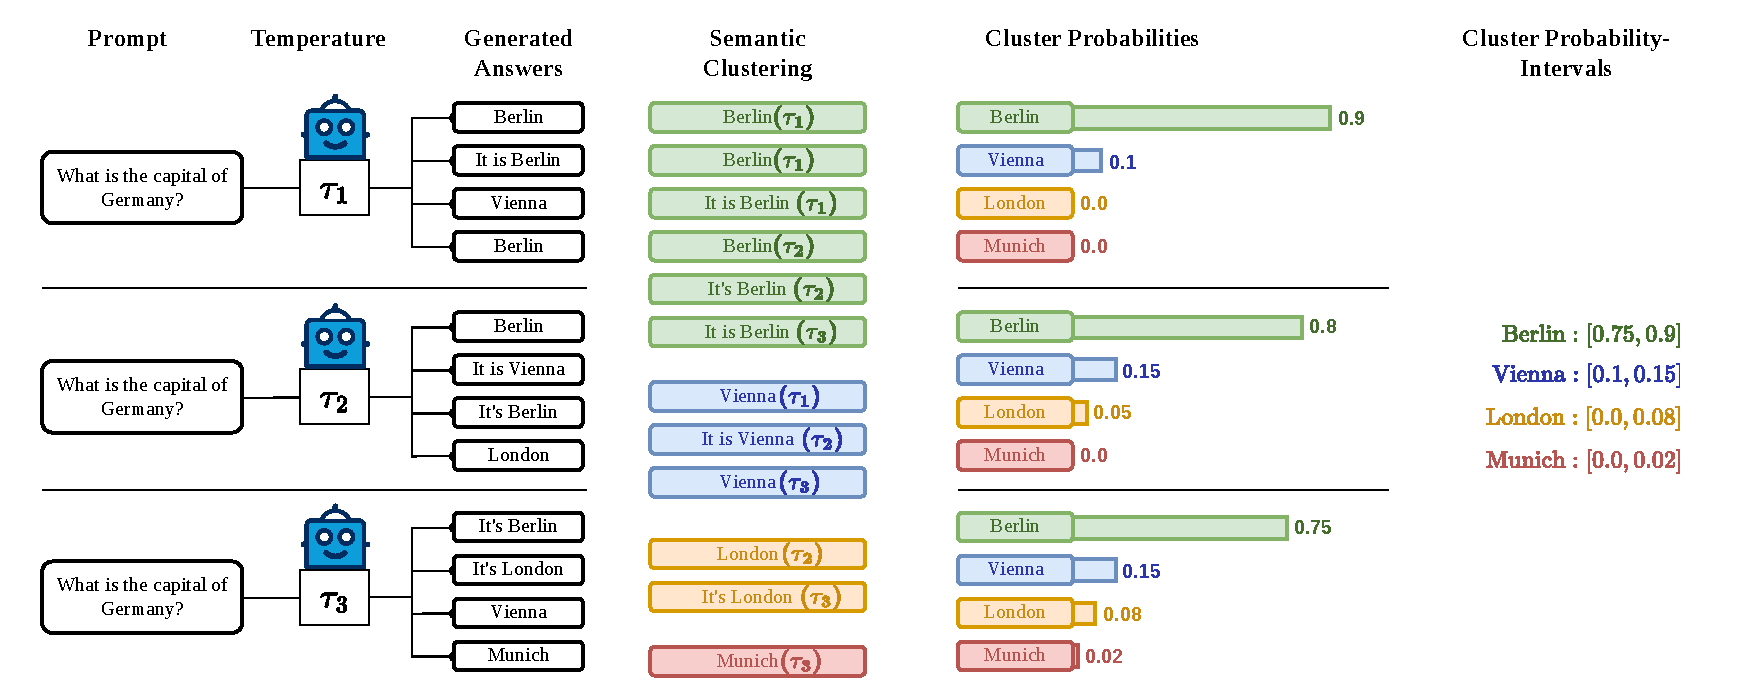
\includegraphics[width=\textwidth]{drawio/CredalSemanticEntropyClusterProbabilities.pdf}
    \caption{Visualization of the first three stages of our 
    methodology. The process 
    begins with multi-temperature generation, followed by semantic 
    clustering performed on the union of all generated sequences. 
    Finally, the probability mass of each cluster is marginalized at 
    every temperature to establish the robust probability intervals 
    used for uncertainty quantification.}
    \label{fig:methodology:pipeline_overview}
\end{figure}

The following sections formally define the mathematical and 
computational mechanics of each stage in this pipeline.




\section{Valid Temperature Selection (the $\alpha-$Cut)}
\label{sec:methodology:temperature_selection}
We consider the task of free-form Question Answering (QA) using a 
pre-trained, autoregressive LLM $\mathcal{M}$ with a vocabulary 
$\mathcal{V}$. This process is performed a priori using a labeled
training dataset or calibration dataset.
We evaluate a predefined grid of candidate temperatures $\mathcal{T}$.
For each temperature $\tau \in \mathcal{T}$, we measure its ability to
assign high probability to the ground-truth answers. This involves
three steps: computing the average NLL, deriving the relative 
likelihood and applying an $\alpha$-cut threshold.

\subsection{Computing the Average Negative Log-Likelihood}
\label{sec:methodology:temperature_selection:average_nll}
For every question-answer pair $(x^{(i)}, \mathbf{y}^{(i)})$ in the 
training dataset $\mathcal{D}_{\text{Train}}$ of size $D$, we compute the 
length-normalized NLL (\ref{eq:average_nll}) of the ground-truth answer 
sequence under the temperature-scaled probability distribution $P^{\tau}$.
The average NLL for a given temperature $\tau$ across the entire 
dataset is computed as: 

\begin{equation}
    \overline{\text{NLL}}(\tau) = 
	\frac{1}{D} \sum_{i=1}^{D} \left( - \frac{1}{T_i} 
	\sum_{t=1}^{T_i} \log P^\tau(y_t^{(i)} \mid 
	\mathbf{y}_{<t}^{(i)}, x^{(i)}) \right)
    \label{eq:temperature_nll}
\end{equation}

where $T_i$ is the length (number of tokens) of the $i$-th target 
sequence. This average NLL serves as our primary metric for evaluating
how well a specific temperature calibrates the model's output 
distribution to the true data distribution. We denote the optimal  
temperature that yields the minimum $\overline{\text{NLL}}$ as $\tau^{ML}$:

\begin{equation}
    \tau^{ML} = \argmin_{\tau \in \mathcal{T}} 
    \overline{\text{NLL}}(\tau)
    \label{eq:temperature_mle}
\end{equation}

\subsection{Deriving Relative Likelihoods}
\label{sec:methodology:temperature_selection:rel_likelihoods}
Because NLL values are absolute and can vary drastically depending
on the model and dataset, it is difficult to define a universal 
threshold for what constitutes a "good" temperature. To standardize
this, we map the average NLLs into the relative likelihood space.

As established in Equation \ref{eq:relative_likelihood},
the relative likelihood $\gamma(\tau)$ of any temperature is computed
by comparing its likelihood $L(\tau)$ to the optimal likelihood 
$L(\tau^{ML})$. In the logarithmic domain, this is equivalent to
to the exponentiated difference of their average NLLs:

\begin{equation}
    \gamma(\tau) = \displaystyle\frac{L(\tau)}{L(\tau^{ML})} 
	= \exp \left( - \left( \overline{\text{NLL}}(\tau) 
	- \overline{\text{NLL}}(\tau^{ML}) \right) \right)
    \label{eq:nll_relative_likelihood}
\end{equation}

By definition, the optimal temperature $\tau^{ML}$ has a relative likelihood
of $\gamma(\tau^{ML}) = 1.0$. All other temperatures $\tau$ will
have a relative likelihood $\gamma(\tau) \in [0,1]$, explicitly
quantifying how plausible they are compared to the best performing 
parameterization.

\subsection{The $\alpha$-Cut}
 \label{sec:methodology:temperature_selection:alpha_cut}
Following the framework of credal prediction 
\cite{löhr2025credalpredictionbasedrelative},
we apply an $\alpha$-cut, retaining only those temperatures whose
relative likelihood meets or exceeds a specified confidence 
threshold $\alpha \in [0,1]$.
The final set of valid temperatures is formally defined as:

\begin{equation}
    \mathcal{T}_\alpha = \{ \tau \in \mathcal{T} : 
    \gamma(\tau) \geq \alpha \}
    \label{eq:temperature_alpha_cut}
\end{equation}


\section{Generation and Semantic Clustering}
\label{sec:methodology:generation}
Once the set of valid temperatures $\mathcal{T}_\alpha$
has been established via the train dataset, we apply the methodology 
to the unseen test queries. For a given input prompt $x$, the goal is
to map the model's raw token outputs into discrete semantic concepts.
This requires a two-step process. Generating a diverse pool of 
candidate responses and clustering them based on semantic equivalence.

\subsection{Multi-Temperature Sequence Generation}
\label{sec:methodology:generation:sequence_generation}
The evaluate the model's uncertainty, we must sample responses from 
every valid temperature.
For each temperature $\tau \in \mathcal{T}_\alpha$, we prompt the 
LLM $\mathcal{M}$ to generate $N$ independent answer sequences.

Let $\mathcal{S}_\tau = \{ s_1^\tau, s_2^\tau, \dots, s_N^\tau \}$ 
denote the set of sequences generated at temperature $\tau$. The total
pool of generated responses for the prompt $x$ is the union of all 
sequences generated across all valid temperatures:

\begin{equation}
    \mathcal{S}_{total} = \bigcup_{\tau \in \mathcal{T}_\alpha} 
	\mathcal{S}_\tau
    \label{eq:pool_of_sequences}
\end{equation}

By generating across $\mathcal{T}_\alpha$, we force the model to 
explore different regions of its probability space. Lower temperatures 
favor the most likely tokens, whereas higher temperatures flatten the 
distribution, encouraging the model to output lower-probability claims.


\subsection{Bidirectional Entailment and Equivalence Classes}
\label{sec:methodology:generation:entailment}
As discussed in Section \ref{sec:related_work:semantic_entropy}, 
evaluating uncertainty on the raw lexical set $\mathcal{S}_{total}$ 
artificially inflates misconfidence due to the aleatoric linguistic 
variations. We therefore partition $\mathcal{S}_{total}$ into a set of 
semantic equivalence classes, or clusters, denoted as 
$C = \{ c_1, c_2, \dots, c_K \}$.

To determine if two distinct sequences $s_i$ and $s_j$ belong to the 
same cluster, we employ an automated Natural Language Inference (NLI)
model (e.g., DeBERTa-large-MNLI 
\cite{he2021debertadecodingenhancedbertdisentangled}).
The NLI model evaluates whether the premise sequence entails the 
hypothesis sequence. We define a strict semantic equivalence relation
$E(\cdot, \cdot)$ which holds true if and only if there is 
\textbf{bidirectional entailment}: 
$(s_i \models s_j) \land (s_j \models s_i)$

If $s_i$ entails $s_j$ and $s_j$ entails $s_i$, the sequences are 
deemed factually equivalent in the context of the prompt $x$ and are 
assigned to the same cluster $c_k$. Thus, a cluster holds all 
sequences  that belong to the same equivalence class of 
$E(\cdot, \cdot)$:  $\forall s, s' \in c_k : E(s, s')$. 
% NOTE: should I leave that in?

\subsection{Constructing the Cluster Probability Distributions}
\label{sec:methodology:generation:cluster_probability}
Once the clusters $C$ are established, we must compute the probability
of each cluster under each temperature $\tau \in \mathcal{T}_\alpha$.
The probability of a semantic cluster $c_k$ at temperature $\tau$ is 
the normalized sum of the likelihoods of all sequences within that 
cluster, evaluated under the distribution $P^\tau$:

\begin{equation}
    P^\tau(C_k \mid x) = 
    \frac{P^\tau(c_k \mid x)}{\sum_{c \in C} P^\tau(c \mid x)}
    \label{eq:normalized_credal_cluster_probs}
\end{equation}

where

\begin{equation}
    P^\tau(c_k \mid x) = \sum_{s \in c_k} P^\tau(s \mid x)
    \label{eq:credal_cluster_probs}
\end{equation}

This marginalization step is crucial. It abstracts away the specific
phrasing of the answers, yielding a set of discrete probability 
distributions $P^\tau(C)$ over the fundamental semantic meaning. 
It is important to note that the set of semantic clusters $C$
is global. It contains every unique meaning generated across 
\textit{all} valid temperatures.
If a specific cluster $c_k$ does not contain any sequences generated 
at a particular temperature $\tau$, we assign it a zero probabilty 
mass for that distribution. This ensures that every distribution 
$P^\tau$ is defined over the same common support $C$, allowing for 
the direct element-wise comparison required to compute the upper and
lower probability bounds in the next step. To compute the sequence
probability $P^\tau(s \mid x)$, we use the length normalized
NLL as defined in Equation \ref{eq:average_nll} because we do not want to
punish longer sequences 
\parencite{malinin2021uncertaintyestimationautoregressivestructured}. 
In the case where shorter answers are wanted, as it is in TriviaQA 
\parencite{joshi2017triviaqalargescaledistantly}, we could use the
unnormalized NLLs (\ref{eq:nll}) as well.

\subsection{Quantifying Credal Semantic Uncertainty}
\label{sec:methodology:uncertainty_quantification}
By scaling the temperature, we observe a range of probabilities for 
each semantic cluster. We utilize the observed probability 
fluctuations to establish upper and lower probability bounds for 
every semantic concept. The \textbf{credal set} is then formally
defined as the set of \textit{all} valid probability distributions 
that respect these element-wise bounds.

\textbf{Establishing Probability Bounds} \\
Let $C = \{ c_1, c_2, \dots, c_K \}$ be the set of identified semantic 
clusters. For each cluster $c_k$, we inspect its probability mass
across all valid temperatures $\tau \in \mathcal{T}_\alpha$
We define the \textbf{lower probability} $\underline{P}(c_k)$ and 
the \textbf{upper probability} $\overline{P}(c_k)$  as the minimum and 
maximum probabilities observed for that cluster. 

\begin{equation}
    \underline{P}(c_k) = \min_{\tau \in \mathcal{T}_\alpha} 
	P^\tau(c_k \mid x)
    \quad \quad
    \overline{P}(c_k) = \max_{\tau \in \mathcal{T}_\alpha}
	P^\tau(c_k \mid x)
    \label{eq:cluster_bounds}
\end{equation}

These bounds define an interval 
$[\underline{P}(c_k), \overline{P}(c_k)]$ representing the model's 
epistemic ambiguity regarding the plausibility of meaning $c_k$.

\begin{figure}
    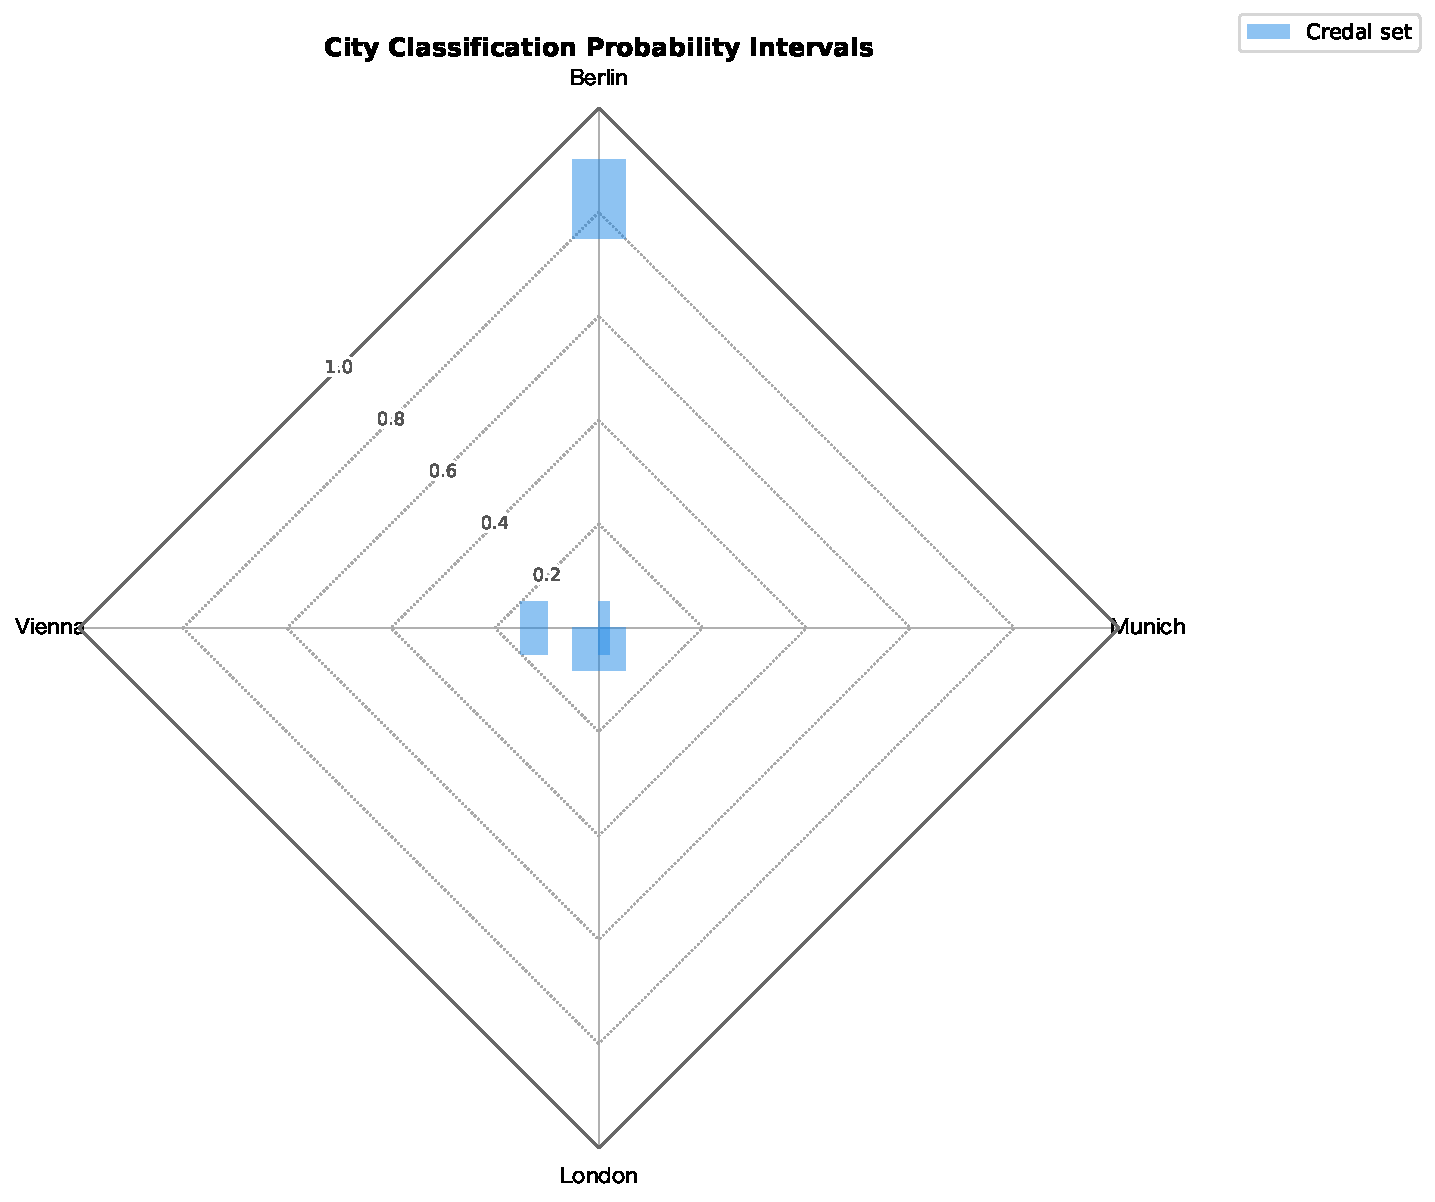
\includegraphics[width=0.7\textwidth]{gfx/city_classification_intervals.pdf}
    \caption{Geometric representation of the credal set derived from the 
    probability intervals established in Figure 
    \ref{fig:methodology:pipeline_overview}. Each axis of the radar chart 
    corresponds to a distinct semantic cluster. The blue bars represent the
    probability intervals (lower to upper bounds) for each class, 
    illustrating the model's epistemic uncertainty across the potential 
    predictions. This visualization approach follows [Hof+26].}
    \label{fig:methodology:visual_probability_bounds}
\end{figure}

\textbf{Defining the Credal Set} \\
We construct the credal set $\mathcal{K}$ as the convex set of all 
probability distributions $P$ over $C$ that are consistent with these
interval bounds. Formally:

\begin{equation}
    \mathcal{K} = \left\{ P \in \Delta_K \mid \forall k: 
	\underline{P}(c_k) \leq P(c_k) \leq \overline{P}(c_k),
	\sum_{k = 1}^K P(c_k) = 1 \right\}
    \label{eq:credal_set}
\end{equation}

where $\Delta_K$ denotes the standard probability simplex. By defining
$\mathcal{K}$ via these bounds, we capture not just the specific 
distributions observed at sampled temperatures, but the entire region 
of probability space supported by the valid relative likelihoods.

\textbf{Upper Semantic Entropy ($H^*$)} \\
This metric corresponds to the maximum entropy (highest uncertainty)
attainable by any distribution within the credal set. It serves as 
our primary signal for hallucination detection 
(\ref{sec:background:credal_sets:uncertainty}), 
identifying cases 
where the model's interval constraints allow for a highly flat, 
uniform distribution:

\begin{equation}
    H^*(x) = \max_{P \in \mathcal{K}} 
	\left( - \sum_{k=1}^K P(c_k) \log P(c_k) \right)
    \label{eq:upper_semantic_entropy}
\end{equation}

\textbf{Lower Semantic Entropy ($H_*$)} \\
Conversely, the lower entropy corresponds to the most deterministic
distribution consistent with the bounds: 

\begin{equation}
    H_*(x) = \min_{P \in \mathcal{K}}
	\left( - \sum_{k=1}^K P(c_k) \log P(c_k)\right)
    \label{eq:lower_semantic_entropy}
\end{equation}

The difference $H^* - H_*$ reflects the magnitude of epistemic 
uncertainty as shown in Section
\ref{sec:background:credal_sets:uncertainty}. 
For the experimental evaluation in this thesis, we utilize the 
upper semantic entropy $H^*$, as it provides the most conservative 
safety guarantee by considering the maximum plausible uncertainty.

    % INCLUDE: methodology
% !TEX root = ../main.tex
%
\chapter{Experiments}
\label{sec:experiments}
To validate the effectiveness of our proposed Credal Semantic
Entropy method, we conducted a series of experiments on a 
standard free-form Question Answering (QA) benchmark.
The primary objective of these experiments is to evaluate
whether quantifying epistemic uncertainty via valid 
temperatures provides a more reliable signal for high uncertainty 
than standard single-point metrics.


\section{Experimental Setup}
\label{sec:experiments:setup}

\subsection{Dataset: CoQA}
\label{sec:experiments:setup:coqa}
We utilized the \textbf{Conversational Question Answering (CoQA)} 
dataset \parencite{reddy2019coqaconversationalquestionanswering}
for our evaluation. CoQA is a large-scale dataset for building
Conversational Question Answering systems. It contains 127k+ 
questions with answers obtained from 8k+ conversations about 
text passages from seven diverse domains 
\parencite{reddy2019coqaconversationalquestionanswering}.

For our specific task, we followed the 
experimental protocol established by 
\textcite{kuhn2023semanticuncertaintylinguisticinvariances}.
We used the development split of CoQA, which provides a diverse 
set of questions. The dataset was split into a \textbf{calibration set} 
(used to determine the valid temperature set) and a \textbf{test set}
(used to evaluate the final uncertainty metrics).


\subsection{Model Architecture}
\label{sec:experiments:setup:model}
All experiments were conducted using the \textbf{Opt-6.7B} model
\parencite{zhang2022opt}. OPT (Open Pre-trained Transformer) is a 
decoder-only architecture that replicates the performance and 
behaviour of GPT-3 \parencite{brown2020languagemodelsfewshotlearners}.
We chose the 6.7B parameter variant as it strikes a balance between
computational feasibility and the capability to generate coherent text.

For the semantic clustering step, we employed a \textbf{DeBERTa-large-MNLI}
model \parencite{he2021debertadecodingenhancedbertdisentangled} to assess
bidirectional entailment between generated answers.

\subsection{Baselines}
\label{sec:experiments:setup:baselines}
We compared our proposed \textbf{Credal Semantic Entropy (Credal SE)}
against several strong baselines:

\begin{itemize}
	\item \textbf{Semantic Entropy (SE)}: The original
	    metric proposed by 
	    \textcite{kuhn2023semanticuncertaintylinguisticinvariances},

	\item \textbf{Lexical Similarity (ROUGE-L)}: We compute the average
	    ROUGE-L score across all pairs of the $N$ sampled sequences.
	    Lower average similarity indicates higher lexical dispersion
	    (uncertainty).
	    \parencite{lin-2004-rouge}.

	\item \textbf{Predictive Entropy (PE)}: The standard entropy of the 
	    model's output distribution over the sequence of tokens.
	    Unlike semantic entropy, this metric considers every lexical 
	    variation as a distinct outcome, calculating uncertainty
	    directly on the raw strings without semantic clustering
	    \parencite{malinin2021uncertaintyestimationautoregressivestructured}.

	\item \textbf{Length-Normalized PE}: A variant of Predictive Entropy
	    that normalizes the sum of token entropies by the sequence 
	    length, mitigating the bias against longer answers
	    \parencite{malinin2021uncertaintyestimationautoregressivestructured}.

	\item \textbf{Margin Measure (MM)}: The difference in
	    log-probability between the most likely sequence and the second
	    most likely sequence. A small margin indicates high uncertainty
	    between the top two choices \parencite{lin-etal-2022-towards}.

	\item \textbf{P(true)}: A self-evaluation metric 
	    \parencite{kadavath2022languagemodelsmostlyknow} 
	    where the model is prompted with the question and its generated
	    answer, and asked to output ``True'' or ``False''. We extract the
	    probability mass assigned to the ``True'' token.
\end{itemize}

\subsection{Evaluation Metric: AUROC}
\label{sec:experiments:setup:evaluation}
To quantify the performance of each uncertainty method, we treat
uncertainty quantification as a binary classification problem. The core
task is to determine if the uncertainty score can reliably distinguish
between correct and incorrect model generations. We use the answers
that were generated by the model using the temperature with the 
maximum likelihood.

\textbf{Ground Truth Labeling} \\
To establish the ground-truth labels for our experiments, we compare 
the generated answers against the gold-standard reference answer 
provided in the CoQA dataset. We define correctness based on lexical 
overlap using the \textbf{ROUGE} metric (Recall-Oriented Understudy 
for Gisting Evaluation) 
\parencite{lin-2004-rouge}. Specifically, a generated answer is 
labeled as:

\begin{itemize}
	\item \textbf{Correct}: If the ROUGE-L score between the 
	    generation and the reference is strictly greater than $0.3$.

	\item \textbf{Incorrect}: If the ROUGE-L score is less than or 
	    equal to $0.3$.
\end{itemize}

This threshold allows for minor phrasing differences while ensuring
that the core semantic content overlaps significantly with the reference.

\textbf{AUROC Calculation} \\
We report the 
\textbf{Area Under the Receiver Operating Characteristic curve (AUROC)}
\parencite{BRADLEY19971145}.
The AUROC represents the probability that a randomly selected incorrect 
answer will have a higher uncertainty score than a randomly 
selected correct answer.

\begin{itemize}
    \item $\text{AUROC} = 0.5$: Indicates random performance 
	(no better than a coin flip)

    \item $\text{AUROC} = 1.0$: Indicates perfect detection 
	(all incorrect answers have higher uncertainty scores than all 
	correct answers).
\end{itemize}

\section{Results}
\label{sec:experiments:results}
As discussed in the methodology, constructing a credal set via 
multi-temperature-sampling incurs significant computational overhead.
To maintain a feasible evaluation pipeline while ensuring sufficient
granularity, we restricted our analysis to the temperature interval
$[0.4, 2.2]$ evaluated at two distinct resolutions:  
a 20-step grid (Table \ref{tab:twenty_steps_interval}) and a 
50-step grid (Table \ref{tab:fifty_steps_interval}).

Our evaluation is conducted on a subset of approximately 2400 queries, using
60\% ($\approx 1440$ questions) of the questions to find valid
temperatures and the other 40\% ($\approx 960$ questions) to evaluate our 
uncertainty estimation, from the CoQA development set.
In this section, we systematically present the
uncertainty quantification performance (measured using AUROC) across
these configurations, exploring how the grid resolution and the relative
likelihood threshold $\alpha$ impact the robustness of our uncertainty
estimates.


\subsection{Evaluation: 20-Step Interval}
\label{sec:experiments:results:twenty_steps_interval}
We begin our analysis using the coarser 20-step temperature interval 
combined with a highly restrictive relative likelihood threshold of 
$\alpha=0.9$. Table \ref{tab:results_20_steps_alpha07} summarizes
the AUROC scores for our proposed Credal Semantic Entropy alongside 
the established single-point baselines. The baselines were evaluated on
the generations predicted by the model using the most likely temperature 
($\tau = 1.347$).

Table \ref{tab:results_20_steps_alpha07}: 
	Hallucination detection performance (AUROC) on the CoQA subset
	using a 20-step temperature interval and a strict relative
	likelihood threshold ($\alpha=0.9$). Metrics compared are our
	proposed Credal Semantic Entropy (Credal SE), standard Semantic
	Entropy (SE), Predictive Entropy (PE), length-normalized Predictive
	Entropy (ln PE), Margin Measure (MM), P(true) and
	Lexical Similarity (LS).
\begin{table}[h]
    \centering
    \begin{tabular}{lccccccc}
        \toprule
	\textbf{Configuration} & \textbf{Credal SE} & \textbf{SE} & \textbf{PE} & \textbf{ln PE} & \textbf{MM} & \textbf{P(true)} &\textbf{LS}\\
        \midrule
    20 Steps, $\alpha = 0.7$ & 0.60 & 0.61 & 0.58 & 0.66 & 0.57 & 0.59 		&\textbf{0.70}\\
        \bottomrule
    \end{tabular}
    \caption{}
    \label{tab:results_20_steps_alpha07}
\end{table}

\begin{figure}
    \center
    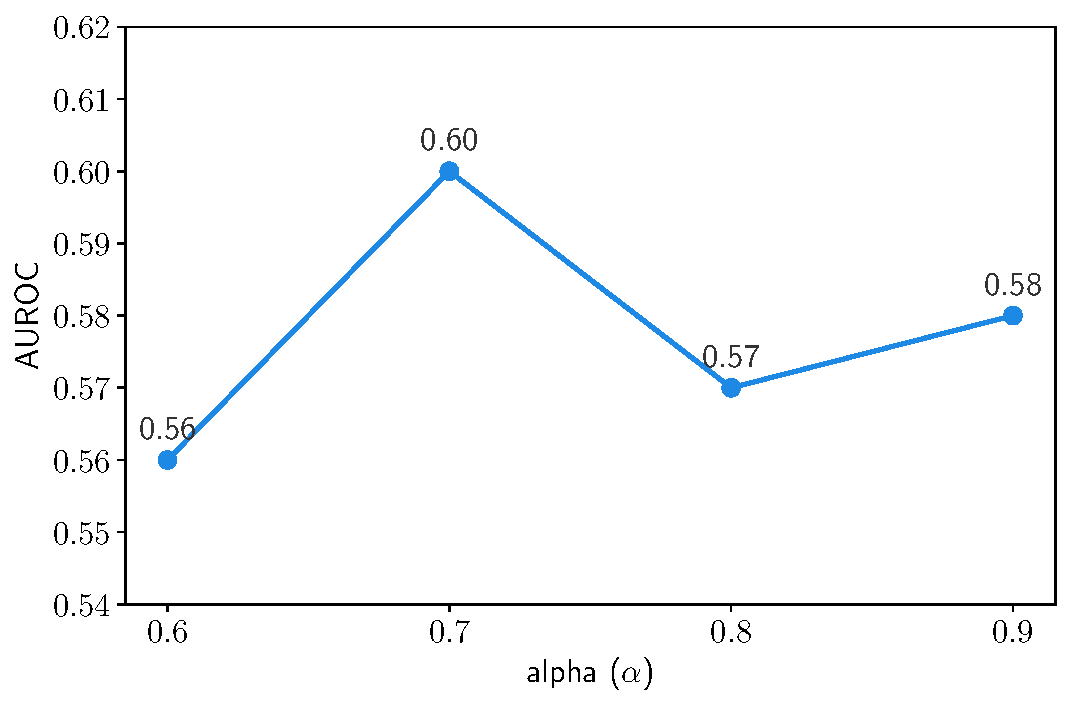
\includegraphics[width=0.6\textwidth]{gfx/alpha_results_lineplot_20_steps.pdf}
    \caption{Impact of the relative likelihood threshold ($\alpha$) on
    the uncertainty quantification performance of 
    Credal Semantic Entropy.
    The line plot illustrates the AUROC scores evaluated on the 20-step
    temperature grid for $\alpha \in \{0.6, 0.7, 0.8, 0.9\}$.}
    \label{fig:experiments:aurocs_alphas_20_steps}
\end{figure}

\textbf{Analysis of 20-Step Results} \\
Under this specific configuration, Lexical Similarity (LS) achieves the
strongest performance with an AUROC of 0.70, followed by length-normalized
Predictive Entropy (ln PE) with 0.66.
Our proposed Credal Semantic Entropy yields an AUROC of 0.58, which
underperforms standard Semantic Entropy (0.61) and equals raw Predictive 
Entropy (0.58).


\subsection{Evaluation: 50-Step Interval}
\label{sec:experiments:results:fifty_steps_interval}
To investigate whether a finer resolution of the temperature space 
improves the calibration of our credal set, we extend our analysis to the
50-step interval (Table \ref{tab:fifty_steps_interval}). As in the previous
experiment, we first evaluate the most restrictive threshold, $\alpha=0.9$.

Table \ref{tab:results_50_steps_alpha09}:
	Hallucination detection performance (AUROC) on the CoQA subset
	using a 50-step temperature interval and a strict relative
	likelihood threshold ($\alpha=0.9$). Metrics compared are our
	proposed Credal Semantic Entropy (Credal SE), standard Semantic
	Entropy (SE), Predictive Entropy (PE), length-normalized Predictive
	Entropy (ln PE), Margin Measure (MM), P(true) and
	Lexical Similarity (LS).
\begin{table}[h]
    \centering
    \begin{tabular}{lccccccc}
        \toprule
	\textbf{Configuration} & \textbf{Credal SE} & \textbf{SE} & \textbf{PE} & \textbf{ln PE} & \textbf{MM} & \textbf{P(true)}
			    &\textbf{LS}\\
        \midrule
	50 Steps, $\alpha = 0.9$ &0.56 &0.62 &0.55 &0.65 &0.54 &0.62
			    &\textbf{0.68}\\
        \bottomrule
    \end{tabular}
    \caption{}
    \label{tab:results_50_steps_alpha09}
\end{table}

\textbf{Analysis of 50-Step Results} \\
Table \ref{tab:results_50_steps_alpha09} demonstrates that under the 50-step
configuration at $\alpha=0.9$, lexical similarity (LS)
maintains its position as the strongest baseline with an AUROC of o.68,
again followed by length-normalized Predictive Entropy (ln PE).
Standard Semantic Entropy (SE) and P(true) perform competitively at 0.62.

Crucially, our proposed Credal Semantic Entropy yields an AUROC of 0.56. 
Notably, this is a slight degradation compared to its performance on the 
coarser 20-step grid (0.58).
Note that we were not able to test more 
$\alpha$ values for the 50-step interval as it was
computationally prohibitive.


\subsection{Additional Evaluation: Local Analysis at $\tau=0.5$}
\label{sec:experiments:results:additional}
In our primary evaluations, the single-point baselines were evaluated at
$\tau \approx 1.39$, as this was the temperature that maximized the average 
likelihood of the calibration data ($\tau^{ML}$). However, 
\textcite{kuhn2023semanticuncertaintylinguisticinvariances} reported that
standard semantic entropy achieves peak performance at a significantly lower
temperature, specifically $\tau=0.5$.
To ensure a fair and comprehensive comparison against this baseline, we 
conducted an additional evaluation centered around this lower temperature
regime.

\textbf{Methodological Caveat: Local Relative Likelihood} \\
Applying our framework strictly, a temperature of $\tau=0.5$ possesses a 
global relative likelihood close to zero when compared to the true optimum
at $\tau \approx 1.39$, and would thus be excluded by any reasonable 
$\alpha$-cut. Consequently, for this specific evaluation, we compute a
\textit{local} relative likelihood. We restricted our grid to a narrow
15-step interval around the baseline's optimum, specifically 
$[0.490, 0.505]$ with a step size of 0.001. Within this local grid, the
maximum likelihood was observed at $\tau=0.505$. Applying an 
$\alpha$-threshold of 0.9 yielded a valid temperature set of 
$\mathcal{T}_{0.9} = \{0.497, 0.498, \dots, 0.505\}$.

\textbf{Results} \\
Table \ref{tab:results_opt_sem_entropy}:
	Hallucination detection performance (AUROC) on the CoQA subset
	using a 15-step temperature interval and a strict relative
	likelihood threshold ($\alpha=0.9$). Metrics compared are our
	proposed Credal Semantic Entropy (Credal SE), standard Semantic
	Entropy (SE), Predictive Entropy (PE), length-normalized Predictive
	Entropy (ln PE), Margin Measure (MM), P(true) and
	Lexical Similarity (LS).
\begin{table}[h]
    \centering
    \begin{tabular}{lccccccc}
        \toprule
	\textbf{Configuration} & \textbf{Credal SE} & \textbf{SE} & \textbf{PE} & \textbf{ln PE} & \textbf{MM} & \textbf{P(true)} &\textbf{LS}\\
        \midrule
    15 Steps, $\alpha = 0.9$ & 0.67 & \textbf{0.74} & 0.64 & 0.72 & 0.61 & 0.69 &0.61\\
        \bottomrule
    \end{tabular}
    \caption{}
    \label{tab:results_opt_sem_entropy}
\end{table}

Under this configuration, Semantic Entropy (SE) achieves the 
highest overall AUROC of 0.74, closely followed by 
length-normalized Predictive Entropy (0.72). Our proposed Credal Semantic
Entropy achieves a score of 0.67, outperforming raw Predictive Entropy 
(0.64) and Lexical Similarity (0.61), but falling short of the leading 
baselines.

\section{Discussion}
\label{sec:experiments:discussion}
The empirical evaluation of Credal Semantic Entropy
presents a nuanced picture of uncertainty quantification
in LLMs. While the credal framework offers a mathematically
rigorous approach to modelling epistemic uncertainty,
translating this theoretical advantage into improved
uncertainty quantification proves challenging in practice.

Across nearly all configurations, single-point baselines, 
particularly length-normalized Predictive Entropy (ln PE) and
Semantic Entropy, demonstrated superior performance.
In the 20-step evaluation (\ref{tab:results_20_steps_alpha07}),
Lexical Similarity achieved the highest AUROC (0.70). 
This suggests that for the OPT-6.7B model on the CoQA dataset,
simple string-level variation across sampled answers is an
exceptionally strong proxy for model ignorance.

As illustrated in Figure \ref{fig:experiments:aurocs_alphas_20_steps},
the performance of Credal Semantic Entropy is highly 
volatile with respect to the $\alpha$-cut.
The line plot reveals a distinct peak at $\tau = 0.7$ (AUROC = 0.60),
with performance degrading when the threshold is made either
stricter ($\alpha = 0.9$) or more permissive ($\alpha = 0.6$).

This behaviour aligns with the geometry of credal sets. A highly 
restrictive threshold ($\alpha = 0.9$) strips the credal set of
meaningful distributional diversity, collapsing the probability
bounds into a noisy point estimate. Conversely, a threshold
that is too loose ($\alpha = 0.6$) introduces ``garbage''
temperature-distributions that are poorly calibrated to the data.
The peak at $\alpha = 0.7$ captures genuine epistemic uncertainty 
without admitting uncalibrated noise. 

Intuitively, evaluating a denser temperature grid should yield
a more accurate approximation of the credal set. However,
our comparison between the 20-step and 50-step intervals
reveals the opposite: performance degraded from 0.58 to 0.56
(at $\alpha = 0.9$). A plausible explanation for this discrepancy
lies in the discrete selection of the maximum likelihood 
temperature ($\tau^{ML}$). As shown in Section 
\ref{sec:experiments:results:additional}, almost all baseline 
UQ methods demonstrate superior performance at lower temperatures
(e.g. $\tau=0.5$). Because the coarser 20-step grid is restricted
to fewer evaluation points, it isolates $\tau^{ML}=1.347$,
which consequently shifts the boundaries of the resulting 
$\alpha$-cut downward. This inadvertently forces the credal set
to encompass lower, higher-performing temperatures, thereby
inflating the overall evaluation metrics.

This grid-resolution artifact serves as a clear symptom of a much
broader, fundamental tension within our methodology: the 
misalignment between predictive likelihood and uncertainty 
quantification.
Our framework constructs the credal set around $\tau \approx 1.39$
because this temperature strictly maximizes the likelihood
of the calibration data. However, the empirical results show
that uncertainty metrics perform much better at uncertainty 
quantification at a significantly lower temperature 
($\tau = 0.5$, where SE achieves 0.74 AUROC).
The temperature that best explains the 
empirical distribution of the text (maximum likelihood)
is not the temperature that separates factual knowledge
from high uncertainty. Because our Relative Likelihood
criterion inherently anchors the credal set to the 
high-temperature, maximum likelihood regime, it forces 
the evaluation into a parameter space where uncertainty 
quantification is more difficult.

Ultimately, while upper semantic entropy over a credal
set captures worst-case uncertainty bounds,
it effectively acts as a measure of \textit{total}
uncertainty. Because it does not explicitly disentangle 
and subtract the aleatoric component, it removes the
advancement over the single-point estimate baselines.
% INCLUDE: experiments
% !TEX root = ../main.tex
%
\chapter{Conclusion}
\label{sec:conclusion}


\section{System Section 1}
\label{sec:conclusion:sec1}


\section{System Section 2}
\label{sec:conclusion:sec2}


\section{Future Work}
\label{sec:conclusion:future}
It would be interesting to see how this method performs on other tasks,
like TriviaQA \parencite{joshi2017triviaqalargescaledistantly}, 
SQuAD \parencite{rajpurkar2018knowdontknowunanswerable} or some medical
or legal dataset like medQA \parencite{jin2020diseasedoespatienthave}
where epistemic uncertainty carries higher risk
and also when implemented using better models, like 
GPT 5 \parencite{singh2025openaigpt5card} or 
Gemini \parencite{geminiteam2025geminifamilyhighlycapable}.
Another interesting strategy would be to not only focus on the 
temperature but on the decoding method itself. By sampling answers 
using Beam Search, Nucleus (Top-p) sampling 
\parencite{holtzman2020curiouscaseneuraltext}, 
Top-k sampling \parencite{fan2018hierarchicalneuralstorygeneration} 
and temperature sampling could also be another interesting method.
     % INCLUDE: conclusion

% --------------------------
% Back matter
% --------------------------
\appendix\cleardoublepage
% !TEX root = ../main.tex
%
\chapter{Appendix}
\label{sec:appendix}

\section{Experimental Details}
\label{sec:appendix:exp_details}

Our implementation builds upon the codebase provided by 
\textcite{kuhn2023semanticuncertaintylinguisticinvariances}. 
We utilize the HuggingFace Transformers library to implement 
both the generative model (OPT-6.7B, \citealp{zhang2022opt}) and the 
entailment model (DeBERTa-large-mnli, 
\citealp{he2021debertadecodingenhancedbertdisentangled}).

To ensure a fair comparison, we replicate the generation parameters 
used in the baseline studies. The generation process is divided into 
two distinct phases using the \texttt{generate()} function:

\textbf{Primary Answer Generation:}
To produce the model's ``best guess'' prediction 
(which is evaluated against the ground truth), we employ beam search 
with sampling enabled. Specifically, we set the beam size to 5 
(\texttt{num\_beams=5}) and enable multinomial sampling 
(\texttt{do\_sample=True}).

\textbf{Uncertainty Estimation Sampling:}
To generate the diverse set of sequences required for computing 
semantic entropy and our proposed credal metrics, we disable beam 
search (\texttt{num\_beams=1}) and rely solely on multinomial sampling 
(\texttt{do\_sample=True}). Following the findings of 
\textcite{kuhn2023semanticuncertaintylinguisticinvariances}, 
who demonstrated that uncertainty estimation performance saturates 
beyond a small number of samples, we generate $N=10$ stochastic 
sequences per question.

Detailed implementation details and instructions regarding hardware 
requirements, environment setup,
and the exact commands required to reproduce the tables and figures
presented in Section 5 are provided in the repository (
\url{https://github.com/liamhpr/Credal-Prediction-for-LLMs.git}).

The experiments run on one 80GB NVIDIA A100.



For our evaluation, we split the temperature interval $[0.4, 2.2]$ using
20 and 50 steps. The step size stays consistent and the resulting 
temperature spaces can be seen in the two Tables 
\ref{tab:twenty_steps_interval}, \ref{tab:fifty_steps_interval} below.

Table \ref{tab:twenty_steps_interval}:
The temperature interval $[0.4, 2.2]$ split into 20 evenly spaced steps. The
temperature yielding the maximum average likelihood ($\tau^{ML} = 1.347$) is
highlighted in bold. In addition, the resulting $\alpha$-cuts
$\mathcal{T}_\alpha$ with $\alpha \in \{0.6, 0.7, 0.8, 0.9\}$ are shown.
\begin{table}[h]
    \centering
    \begin{tabular}{p{0.85\textwidth}}
    \toprule
    \textbf{Set of Evaluated Temperatures ($\mathcal{T}$)} \\
    \midrule
    0.400, 0.495, 0.590, 0.684, 0.779, 0.874, 0.968, 1.063, 1.158, 
    1.253, \\
    \textbf{1.347}, 1.442, 1.537, 1.632, 1.726, 1.821, 1.916, 2.011, 2.105, 2.200 \\
    \midrule
    $\mathcal{T}_{0.9} = \{ 1.253, \dots, 1.537\}$ \quad \quad
    $|\mathcal{T}_{0.9}| = 4$ \\
    $\mathcal{T}_{0.8} = \{ 1.158, \dots, 1.632 \}$ \quad \quad
    $|\mathcal{T}_{0.8}| = 6$ \\
    $\mathcal{T}_{0.7} = \{ 1.063, \dots, 1.726 \}$ \quad \quad
    $|\mathcal{T}_{0.7}| = 10$ \\
    $\mathcal{T}_{0.6} = \{ 1.063, \dots, 1.821\}$ \quad \quad
    $|\mathcal{T}_{0.6}| = 11$ \\
    \bottomrule
    \end{tabular}
    \caption{}
    \label{tab:twenty_steps_interval}
\end{table}

Table \ref{tab:fifty_steps_interval}:
The temperature interval $[0.4, 2.2]$ split into 50 evenly spaced steps. The
temperature yielding the maximum average likelihood ($\tau^{ML} = 1.392$) is
highlighted in bold. In addition, the resulting $\alpha$-cuts
$\mathcal{T}_\alpha$ with $\alpha=0.9$ are shown.
\begin{table}[h]
    \centering
    \begin{tabular}{p{0.9\textwidth}}
    \toprule
    \textbf{Set of Evaluated Temperatures ($\mathcal{T}$)} \\
    \midrule
    0.400, 0.437, 0.474, 0.510, 0.547, 0.584, 0.620, 0.657, 0.694, 0.731, 
    0.767, 0.804, 0.841, 0.878, 0.914, 0.951, 0.988, 1.025, 1.061, 1.098, 
    1.135, 1.171, 1.208, 1.245, 1.282, 1.318, 1.355, \textbf{1.392}, 1.429, 1.465, 
    1.502, 1.539, 1.576, 1.612, 1.649, 1.686, 1.723, 1.759, 1.796, 1.833, 
    1.869, 1.906, 1.943, 1.980, 2.016, 2.053, 2.090, 2.127, 2.163, 2.200 \\
    \midrule
    $\mathcal{T}_{0.9} = \{ 1.208, \dots, 1.576 \}$ \quad \quad
    $|\mathcal{T}_{0.9}| = 11$\\
    \bottomrule
    \end{tabular}
    \caption{}
    \label{tab:fifty_steps_interval}
\end{table}
       % INCLUDE: appendix
%
{%
\setstretch{1.1}
\renewcommand{\bibfont}{\normalfont\small}
\setlength{\biblabelsep}{0pt}
\setlength{\bibitemsep}{0.5\baselineskip plus 0.5\baselineskip}
\printbibliography[nottype=online]
\newrefcontext[labelprefix={@}]
\printbibliography[heading=subbibliography,title={Webpages},type=online]
}
\cleardoublepage

\listoffigures
\cleardoublepage

\listoftables
\cleardoublepage

\newpage
Ich erkläre hiermit, dass ich die vorliegende Arbeit selbstständig und nur mit den angegebenen Hilfsmitteln verfasst habe. Alle Passagen, die ich aus einer Literatur oder anderen Quellen übernommen habe, sind eindeutig als Zitate mit Quellenangabe gekennzeichnet.
Diese gedruckte Fassung ist ein Ausdruck der eingereichten elektronischen Fassung.

I hereby declare that I have written this work independently and only with the aids specified. All passages that I have taken from literature or other sources have been clearly marked as quotations with reference to the source.
This printed copy is a printout of the submitted electronic copy.\\ \\ \\

$\overline{\text{Datum/date Unterschrift/signature}}$
\cleardoublepage

\input{content/colophon}
\cleardoublepage

\newpage
\mbox{}

% **************************************************
% End of Document CONTENT
% **************************************************
\end{document}
